\documentclass[11pt]{article}
\usepackage[margin=1.1in]{geometry}
\usepackage{amsmath,amssymb,amsthm}
\usepackage{booktabs}
\usepackage{array}
\usepackage{tabularx}
\usepackage[protrusion=true,expansion=false]{microtype}
\usepackage[table]{xcolor}
\usepackage{enumitem}
\usepackage{titlesec}
\usepackage{tikz}
\usepackage{float}
\usetikzlibrary{arrows.meta,positioning,fit,calc,decorations.pathreplacing}
\usepackage{listings}
\usepackage{hyperref}

\hypersetup{colorlinks=true, linkcolor=blue!60!black, urlcolor=blue!60!black, citecolor=blue!60!black}
\usepackage[skip=0.6\baselineskip, indent=0pt]{parskip}

\titleformat{\section}{\large\bfseries}{\thesection.}{0.7em}{}
\titleformat{\subsection}{\normalsize\bfseries}{\thesubsection.}{0.6em}{}

\newcommand{\vmax}{V_{\max}}
\newcommand{\Tc}{T_{\mathrm{close}}}
\newcommand{\tx}[1]{\texttt{#1}}
\newcolumntype{L}{>{\raggedright\arraybackslash}X}

\lstdefinestyle{script}{
  basicstyle=\ttfamily\small,
  columns=fullflexible,
  keepspaces=true,
  breaklines=true,
  frame=single,
  framerule=0.3pt,
  xleftmargin=1em,
  escapeinside={(*}{*)},
}

\newtheorem{assumption}{Assumption}

% tables: a little more room between rows, and every other row shaded, so
% that rows of wrapped text stay distinct
\renewcommand{\arraystretch}{1.3}
\rowcolors{1}{}{black!5}

\definecolor{coop}{RGB}{232,245,233}
\definecolor{chainc}{RGB}{255,228,225}
\definecolor{proofc}{RGB}{230,240,255}

\title{\textbf{Lichen}\\L2s In CHannels ENforced by bitcoin}
\author{waxwing}
\date{Version 0.5, November 2026}

\begin{document}
\maketitle

\begin{abstract}
A \emph{contract} with a hub lets a user hold the hub's tokens on a layer 2 and
withdraw them as bitcoin without trusting the hub for honesty or liveness. The L2 tokens are collateralised by the bitcoin in the user-hub multisig output\footnote{a standalone 2-of-2 output (a channel embedding is possible; Section~\ref{sec:contract})}, and if the hub refuses a withdrawal, or cannot answer because it is offline, it is enforced on Bitcoin. The only assumptions are those of the layer 2 itself. \underline{No change to Bitcoin's
consensus is required}. A withdrawal is a claim; if false, its falsehood is proved by the hub with RISC Zero and wrapped in Groth16, and a thus-disputed claim is settled on Bitcoin by a \emph{verification gadget} that checks the Groth16 proof: the one chosen is BABE~\cite{babe}, using witness encryption and garbled circuits, in two to four transactions (BitVMX~\cite{bitvmx} has also been implemented and tested).  Withdrawals are executed cooperatively in the contract --- the normal case, because the statement is independently verifiable and disputing a true claim costs the hub --- or, otherwise, a refused one is played as a dispute on chain, set up at the start of each contract. The trustlessness gain is paid for with liquidity (with receiving ability only contingent on offered ``inbound'' from the hub, as in Lightning). The hub (but not user) must also stay live during normal operation, since an offline hub loses disputes by timeout. The design is built and measured a privacy-focused, shielded-note ledger~\cite{lichencode,lichenl2}; an ecash design whose hub is the mint~\cite{lichenecash} is under development.
\end{abstract}

\tableofcontents

%\section{Introduction}

\section{Obvious objections to Lichen and why they're mostly wrong}
\label{sec:intro}

\paragraph{One central hub is dangerous.} If the hub disappears, the user gets the money. The hub cannot Sybil attack users by printing tokens fictitiously; the honest users' money is all backed. The only remaining risks are inherent to the L2 itself (is it a validity rollup or a quorum? Does it inherit finality from Bitcoin or is finality weaker? Etc.)

\paragraph{Bridges usually mean you can only withdraw a fixed size utxo, meaning operators and relying on swaps. Surely that applies here?} No. The withdrawal amount is encoded in bits in the bitcoin transaction witness, in dispute. This allows us to withdraw arbitrary amounts via multiple outputs of certain denominations~[\ref{sec:outcomes}].

\paragraph{Don't these constructions usually require a 1 of n honesty assumption from a signing committee?} Not here: we avoid this by the LN-GAP~\cite{lngap} trick: the contract is a \emph{bilateral} contract between the hub and each user; the presigning happens between them, just as in Lightning.

\paragraph{But if a bunch of users open contracts with a hub, they can just .. pay each other through Lightning channels?} A correct critique, partly, \underline{if} the L2 ledger doesn't do anything but plain payments. Even then, you could avoid receiver liveness being needed, avoid routing and other minor things. But the real answer is: the L2 can offer more functionality. It can offer private payments, smart contracts, etc.

\paragraph{But this is an IOU/ hub's token, so it's not actually bitcoin.} Incorrect with a crucial caveat. See the first point: every sat is redeemable via the user-hub contracts, \emph{without} the hub's permission, via the contract utxo, so these are actually bitcoin \emph{but only as long as you have liquidity to receive them}. A new user on L2 without a contract with the hub, or a user holding a balance on L2 in excess of their inbound liquidity in their own contract, is holding \emph{credit}, and has no such guarantee. But that's their choice.

\paragraph{But still, a single central hub feels like bad design. Why not multiple hubs?} Having multiple hubs \emph{will} make sense --- see Section~\ref{sec:multihub}, but done naively, it is broken. It's because of what these L2 tokens are. They are fungible, \underline{enforceable} claims on the hub's money; they are minted by the hub itself, just on its own say-so. If you had hub 1 and hub 2, those claims are not transferrable trustlessly to the hubs themselves. If hub 2 prints a billion sats out of nothing and users accept it on the L2 they can redeem it with hub1, leaving hub1 out of pocket. From this line of thinking we see an interesting comparison with ecash servers: the hub can print as much as it likes, but it cannot steal/``rug''.

\paragraph{So what's the catch?} The negatives are twofold: one is liquidity, and this is easy to understand as the analog of the inbound liquidity pain point in Lightning, because it's basically the same thing. Such a hub \emph{can} choose to give no inbound liquidity to a user: they get tokens on L2 to spend, but they cannot (safely) receive. If they receive, it's just credit that someone else will hopefully buy from them. But the design does not assume that, of course, it allows receiving up to a ``cap'': the user negotiates that extra potential receiving amount (inbound liquidity) when it sets up the contract with the hub. The second is the on-chain dispute, whose size depends on the gadget: two to four transactions and 2--31~kvB under BABE, lichen's gadget, against tens of transactions and 100--200~kvB under BitVMX (previously tested), both as measured on Mutinynet~\cite{lichenl2,lichenbitvmx}.

\section{Contracts with the hub}
\label{sec:terms}

\textbf{Alice}, the user, has a contract with a \textbf{Hub}, instantiated as a 2 of 2 output  (see Section~\ref{sec:contract} for the possibility of embedding this inside a Lightning channel), with these terms:
\begin{center}
\small
\begin{tabularx}{\linewidth}{p{16mm}L}
\toprule
$D$ & Alice's deposit: she puts $D$ bitcoin in and receives $D$ of the hub's tokens on the L2 \\
$\vmax$ & the most she can withdraw: her $D$ plus the hub's liquidity $\vmax - D$ (which can be zero)\footnotemark\\
$r_A, r_H$ & the \emph{contract reserves}, for fees. Forfeited by losing side of a dispute, otherwise returned to owner. (Section~\ref{sec:outcomes}); the contract holds $\vmax + r_A + r_H$ \\
$b$ & the amount she withdraws, by claiming $b$ tokens in contract $c$ \\
$c$ & the contract's identifier \\
$\Tc$ & the contract's end: with no withdrawal by then, the hub takes it \\
\bottomrule
\end{tabularx}
\end{center}
\footnotetext{A hub can charge for its liquidity: for a fee $f$ it mints Alice $D - f$ tokens, and the cap is $D - f$ plus the liquidity. Nothing below depends on this, so we leave the fee out.}
Every token is a liability of the hub, collateralised by the contract of whoever holds it, within that holder's cap; within $\vmax$ and before $\Tc$, Alice trusts the hub for nothing, not even to be online: a withdrawal it does not answer is paid by timeout.

\paragraph{Opening is atomic.} Alice's $D$ goes into the contract and this entitles her
$D$ tokens on the L2. This must be atomic: a hub
that took the funding and never minted would leave her nothing to
return, and the default at $\Tc$ would hand it her $D$; a hub that
minted first could be left with tokens backed by no contract. Alice
first pays a deposit output\footnote{A well known design pattern to avoid the need for Alice's external wallet to support some kind of co-signing event}, the hub's key and hers together, or hers
alone after a timeout. The hub then mints $D$ to the key
$P = H(A \,\|\, T)\cdot A + T$, where $A$ is Alice's L2 key and $T = t\cdot G$
a point of the funding transaction's own (the coefficient keeps Alice
from choosing $A$ against $T$), and Alice, once she sees that mint
final on L2, signs the funding's deposit input as an adaptor pre-signature
locked to $T$. The hub can lock the deposit only by completing the adaptor,
which publishes $t$ and so unlocks her tokens. The hub's side needs no
refund: if it never broadcasts, Alice refunds the deposit, and the
locked tokens, which cost nothing to print, stay where they are. Its one
risk is timing: $t$ is public once the funding is in the mempool, so it
broadcasts only well before the deposit's refund matures.

\begin{figure}[H]
\centering
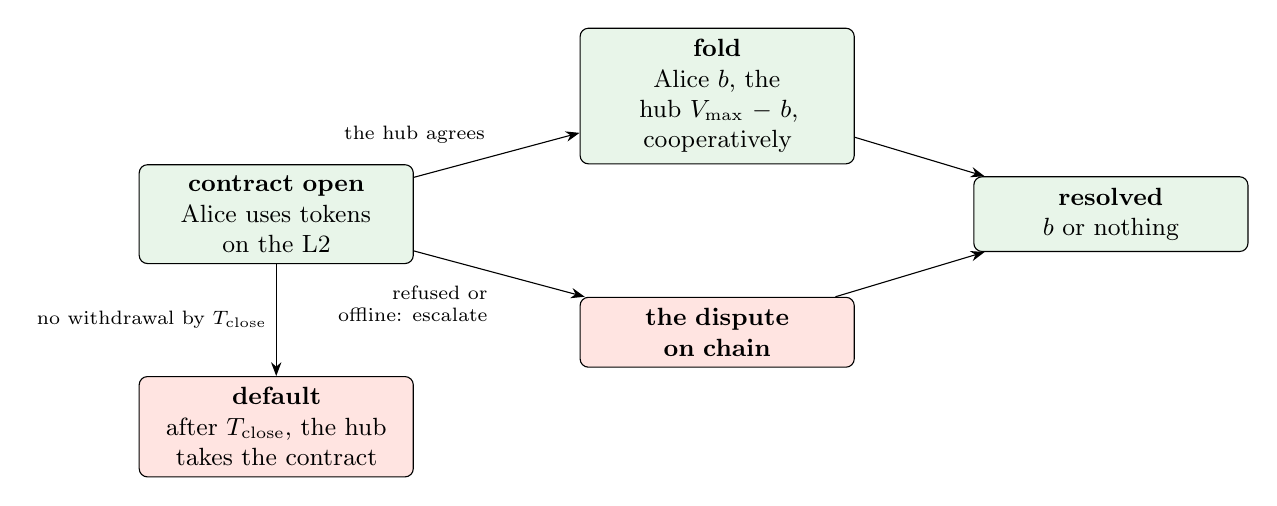
\begin{tikzpicture}[
  font=\small,
  st/.style={draw, rounded corners=3pt, align=center, inner sep=4pt, text width=#1},
  st/.default=32mm,
  >={Stealth[length=5pt]},
]
\node[st, fill=coop] (live) at (0,0) {\textbf{contract open}\\Alice uses tokens\\on the L2};
\node[st, fill=coop] (fold) at (5.6,1.5) {\textbf{fold}\\Alice $b$, the hub $\vmax - b$,\\cooperatively};
\node[st, fill=chainc] (ladder) at (5.6,-1.5) {\textbf{the dispute on chain}};
\node[st, fill=chainc] (def) at (0,-2.7) {\textbf{default}\\after $\Tc$, the hub\\takes the contract};
\node[st, fill=coop] (end) at (10.6,0) {\textbf{resolved}\\$b$ or nothing};
\draw[->] (live) -- node[above left=1pt, font=\scriptsize] {the hub agrees} (fold);
\draw[->] (live) -- node[below left=1pt, font=\scriptsize, align=right] {refused or\\offline: escalate} (ladder);
\draw[->] (live) -- node[left, font=\scriptsize] {no withdrawal by $\Tc$} (def);
\draw[->] (fold) -- (end);
\draw[->] (ladder) -- (end);
\end{tikzpicture}
\caption{The life of a contract. Green states settle
cooperatively (and could remain offchain in channels).}
\label{fig:life}
\end{figure}

\section{How a withdrawal from the L2 is enforced}
\label{sec:statement}

We apply typical optimistic logic: the withdrawal always starts as a \emph{claim}. This way, even if the \texttt{fold} option is not chosen by the hub, the default behaviour is always ``I claim $b$ satoshis, give me the money'' and it is withdrawn without challenge. We prefer a model in which the high-level logic is ``Alice claims, Hub claims proof of incorrectness of claim, Alice challenges proof, proof is resolved with BABE mechanism'' rather than ``Alice claims, Hub co-signs $b$, Alice claims proof of correctness of claim, Hub challenges proof, proof is resolved with BABE mechanism.''

The main advantage of choosing the first over the second is \emph{not} actually onchain space usage, though in many cases it will be smaller. The real advantage is \underline{who proves}. We would like users to mostly act as light clients, in almost all versions of the L2 attached to this verification gadget. This is greatly helped if the proving step only ever has to be done by the Hub, not by the user. Hubs can afford to invest in infrastructure such as dynamically allocated --- i.e. used only in dispute --- GPU proving which can provide orders of magnitude speedup, very economically, in the best cases.

\subsection{The statement proved}

The details of the statement proved will of course depend on the L2's architecture. In abstract, the withdrawal claim can be successfully challenged by the hub, only by a satisfaction of the predicate:

%\[\mathcal{R}_L(\mathcal{D}, c, \ldots ; w=(b, \ldots))\]

\[
\mathcal{R}_H\big(\mathcal{D}, c, \ldots;\; w = (\mathsf{req}, \rho, \ldots)\big)
\;=\; \neg\,\mathsf{Valid}_L\big(C(\mathsf{req}),\, b(\mathsf{req})\big),
\]

where $\mathsf{req}$ is the user's request as confirmed on Bitcoin\footnote{This isn't \emph{necessarily} a presigned input; in some cases it can be confirmed published in advance, and tied in with an inclusion proof}, carrying
her claim $C$ and the amount $b$ she signed, and $\rho$ represents the \emph{refutation}:
evidence, from data the hub holds, that the claim is false. 

Only the public
input $(\mathcal{D}, c, \ldots)$ is fixed when the contract opens; the claim
enters through the witness, authenticated by Bitcoin, which checked the user's
signatures when $\mathsf{req}$ confirmed.

What counts as a refutation is the L2's to define (hence the $L$ subscript). It may be intrinsic to the
claim, i.e. an inherent contradiction, or it might be a fact about the L2's state evolution. If the latter, it needs a notion of time: the state must be fixed relative to
$\mathsf{req}$, so that the operator cannot change it after seeing the claim.
The L2 must ensure that an honest claim admits no refutation; in particular,
a payment whose fate the claimant cannot yet know must not be usable against
her. Where that cannot be arranged, the claim may carry fallback amounts, and
the hub prove only that it is worth less than $b$\footnote{This additional complexity turns out to be relevant to ecash designs, in particular}.

\subsection{L2 examples}

\begin{itemize}
\item An L2 managed by a large quorum with threshold signing of some form (here you'd be trusting the signers for L2 updates, not for withdrawals; arguably not a compelling model since they can block transfers on L2, so they have to be trusted with the money, like any federated/quorum model)
\item An L2 that handles ecash notes where the hub is the mint, requiring extra tricks to make the hub trustless (such as the design in~\cite{lichenecash})
\item an L2 hosted on another blockchain such as Ethereum
\item an L2 using a single use seal on Bitcoin itself to achieve finality and validity proofs of state transition (such as our own design described in~\cite{lichenl2})
\end{itemize}

\ldots the degree to which trustless exit can be claimed will vary, but that is a matter for the L2 architecture: \underline{lichen simply enforces the L2's ruleset, and that part \emph{is} trustless}.

In the remainder of Section~\ref{sec:statement}, we will focus on the mechanical details by which this is achieved.

\subsection{From a program to a verifiable claim}

\begin{figure}[H]
\centering
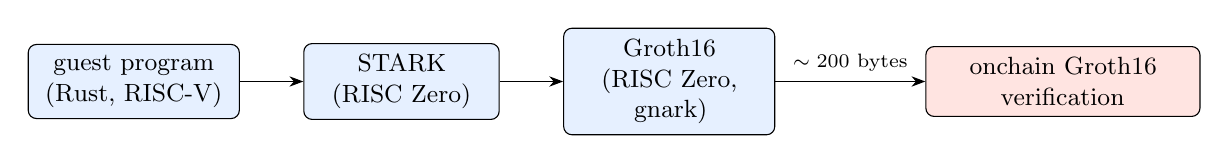
\begin{tikzpicture}[
  font=\small,
  box/.style={draw, rounded corners=3pt, align=center, inner sep=4pt, text width=#1},
  box/.default=27mm,
  >={Stealth[length=5pt]},
]
\node[box=24mm, fill=proofc] (g) at (0,0) {guest program\\(Rust, RISC-V)};
\node[box=22mm, fill=proofc] (s) at (3.4,0) {STARK\\(RISC Zero)};
\node[box=24mm, fill=proofc] (w) at (6.8,0) {Groth16\\(RISC Zero, gnark)};
\node[box=32mm, fill=chainc] (v) at (11.8,0) {onchain Groth16\\verification};
\draw[->] (g) -- (s);
\draw[->] (s) -- (w);
\draw[->] (w) -- node[above, font=\scriptsize] {$\sim200$ bytes} (v);
\end{tikzpicture}
\caption{The hub's withdrawal statement counter-proof runs in RISC Zero's zkVM; its proof is
compressed to a Groth16 proof, which the verification gadget checks on
Bitcoin (Section~\ref{sec:blocks})~\cite{risc0}. An explainer covers each
stage~\cite{pipeline}.}
\end{figure}

\paragraph{What the contract must bind.} The hub's proof must be tied to
three things: the program, since a valid proof of another program proves
nothing; this contract, so that a proof made for another contract or
deployment fails; and the claim it answers, so that the hub cannot refute
a claim other than the one Alice posted. With RISC Zero, the proof's
public input is a digest of the program's image id and its journal (RISC Zero's Groth16 circuit proves only that some STARK verifies, and its
verifying key is the same for every program; a program is identified only
by its image id, hashed into the public input with the journal. So the
contract must fix the image id there, or a valid proof of any program
would do). Under BABE the whole public input is fixed
when the contract is set up: the image id of the hub's statement, and a
journal committing to the contract $c$ and the deployment $\mathcal{D}$
(its keys and any other parameters the statement needs). The claim cannot
be fixed in advance, so it enters through the witness, and the statement
must authenticate it as the one in Alice's \texttt{request}. Her claim and
the amount $b$ are under one-time signatures, which Script verified when
\texttt{request} confirmed; the statement can either check them itself, or
read \texttt{request} from Bitcoin, which it must do anyway if the L2
judges claims as of the time they were made. The same signature on $b$ is
what the payout's bit outputs read (Section~\ref{sec:outcomes}).


\section{Settling a dispute on Bitcoin}
\label{sec:blocks}

The contract is a single taproot output, 2-of-2 between Alice and the
hub with three spending leaves. Transactions pre-signed at
opening let either party carry out its side of a dispute without the
other. What settles a dispute is the on-chain \emph{verification gadget}; in concrete, here, it is always BABE, but we did earlier implement BitVMX to validate the mechanism with an alternative gadget~\cite{lichenbitvmx}.

The idea is, whatever the verification gadget, BitVMX, BABE or other, given a (counter-)proof whose input binds the
program's context ($c , \mathcal{D}, b \ldots )$ as mentioned above, adjudicate the
claim on Bitcoin. The context is checked, the amount $b$ is read into Script, and the loser pays. To emphasize: this is all verification. The proving side, up to the Groth16 proof, is the same whichever gadget is used \footnote{Caveat: this may not be entirely true, depending. For example, our BABE usage requires authenticating $b$ as part of the proof.}.

\subsection{Values that Script can read: one-time signatures}

Bitcoin Script can check a signature only on the spending transaction,
never on a message of the signer's choosing. A contract that must act on
a value a party chooses later, above all Alice's amount $b$, may use Winternitz
one-time signatures, which Script verifies by hashing alone, leaving the
signed digits on the stack to compare~\cite{bitvm,bitvmx}. The keys are
exchanged when the contract opens, one per value, each used once;
signing two different values under one key is \emph{equivocation},
which a leaf can prove, giving the signer's stake to its counterparty.

\subsection{The first gadget: BitVMX}

The first experiments, using a different client-proves algorithm (substantially similar except in who makes the ZKP), were done with BitVMX~\cite{bitvmx}, a heavier but simpler mechanism than BABE. BitVMX settles a claim about a RISC-V program's run by an
interactive search over its execution. In those experiments, Alice claimed that the Groth16
verifier, run on her signed input, halted with success; if the hub
disagreed, they narrowed the run down, eight segments a round, to a single
step, which Alice then proved in Script or the hub disproved. Each move
was a pre-signed transaction carrying the mover's one-time signatures,
and a lie about a memory read was caught through an authenticated jump
list instead of a second search. The companion
paper~\cite{lichenbitvmx} gives the transaction graph and the
measurements from tests that were carried out on regtest and Mutinynet.

\subsection{Lichen's current gadget: BABE with authenticated amounts}

BABE~\cite{babe} replaces the search with a challenge. In making this change, we have also switched to a hub-proves algorithm as was outlined in Section~\ref{sec:statement}.

At setup, the user Alice
garbles a small circuit that turns the first group element of the Hub's (Groth16) invalidity proof
into the key of a witness encryption, so that only a valid proof unlocks
the message it needs to be paid. The Hub posts that element, signed; if
Alice challenges, she must reveal the circuit's input labels for it,
and with a valid proof the Hub decrypts and posts the now-decrypted message. Against an
Alice that garbles wrongly, the Hub checks the garbling by cut-and-choose: Alice makes 78 instances, the Hub opens 68 and keeps 10, and lichen replaces BABE's soldering with verifiable secret sharing, taking the design from Glock~\cite{glock}. Setup then costs about a minute per contract: Alice garbles the 78 instances in under ten seconds on a laptop and uploads the 10 kept ones, about 240~MiB, which the hub stores; the hub checks the other 68 in 20 to 36 seconds. BABE's obstacle is
that the statement is fixed at setup, while Alice chooses $b$ (or more generally, her claim $C$) only when
she withdraws. The claim and amount therefore move into the witness, together with
Alice's one-time signature on them, which she must give onchain to instantiate the claim. This is our
proposal~\cite{delving} (or rather, a slight variant of it, since we have changed to hub-proves not Alice-proves and so don't need the second Winternitz signature, from the hub). Unlike GOAT's cryptographic
alternative~\cite{goat}, in our proposal, BABE's cryptography is
unchanged. It is built as lichen's default gadget.
Appendix~\ref{app:babe} gives the construction as built, and the
companion paper~\cite{lichenl2} the measurements.

\begin{table}[!htp]
\centering
\small
\begin{tabularx}{\linewidth}{>{\raggedright\arraybackslash}p{58mm}LL}
\toprule
& BitVMX & BABE \\
\midrule
a withdrawal the hub never answers & 23~kvB, 5 transactions & 2.7~kvB, 2 \\
a true claim refused, played to the end & ${\sim}120$~kvB, 23 transactions & 2.7~kvB, 2; 31.2~kvB, 4 if the hub asserts a false proof \\
a false claim & 100--200~kvB & 9.9~kvB, 3, if Alice concedes; 30.8~kvB, 4, if she challenges \\
the worst case & ${\sim}200$~kvB (a lie about a read) & 31.2~kvB \\
pre-signed per contract & 141 transactions & 17 \\
setup per contract, beyond pre-signing & none & about a minute; ${\sim}240$~MiB uploaded by the user, stored by the hub \\
contracts a hub can hold, disputes lasting a week\textsuperscript{*} & 3,300 (8,350 with a window per move) & ${\sim}35{,}000$ (est.) \\
\bottomrule
\end{tabularx}
\caption{The two gadgets, as measured on Mutinynet but where marked~\cite{lichenbitvmx,lichenl2}.
\textsuperscript{*}Before congesting the chain becomes a profitable
attack: for $N$ contracts, every move due within a window of $w$ blocks
must fit in it, $N s \le w \cdot 1\,\mathrm{MvB}$~\cite{floodloot}, and
the dispute lasts the sum of its windows. For BABE the windowed moves are
the hub's \tx{assert}, Alice's \tx{challenge\_assert} and the hub's
answer, 28.7~kvB in all, against a week of mainnet blocks.}
\label{tab:gadgets}
\end{table}

\section{The contract logic}
\label{sec:contract}

\subsection{Three ways out}

A contract ends in one of three ways; its output carries three leaves (not including a revocation if inside a channel):
\begin{itemize}[leftmargin=1.5em]
\item the \emph{fold}: a cooperative close of the contract (Alice
  $b + r_A$, the hub $\vmax - b + r_H$), the normal case, nothing on
  chain;
\item \tx{default}: after $\Tc$, a transaction pre-signed at the
  contract's opening pays the hub $\vmax + r_H$ and returns Alice's
  reserve $r_A$. This is the liveness requirement on Alice: turn up at the end, i.e. it's a very low bar requirement; whereas the hub must always be ready to answer disputes.
\item \tx{request}: Alice's claim goes on chain
  as the first step of the dispute.
\end{itemize}

\paragraph{On its own, or in a channel?} A contract is a standalone
output, a 2-of-2 between Alice and the hub, opened by one on-chain
transaction and folded by another. This is the design as built, and the
one this paper assumes. The same output could sit in a Lightning channel
commitment, making the fold a channel update and letting deposits arrive
as Lightning payments, as earlier LN-GAP code demonstrates. But the
price is high. Every channel update re-signs the contract's pre-signed
transactions for both commitments (17 each under BABE, 141 under
BitVMX); renewal,
though off chain, is still a new contract and, under BABE, a new setup;
and a channel's revoked states bring back the always-on watchtower that a
standalone contract avoids. Since we have switched to BABE as our main verification gadget, this option becomes less attractive unless some new engineering is possible to reduce the setup cost.
\subsection{Outcomes}
\label{sec:outcomes}

The dispute only ever decides Alice's withdrawal: in most L2 designs, that's a simple binary: $b$ if her claim
stands, nothing if it fails. The amount analysis that follows assumes that that binary structure applies:

The rest of $\vmax$ goes to the hub. The
reserves follow the dispute: the loser's goes to the winner, whether
it lost on the merits, by signing two values of $b$ (\tx{equiv\_b}), or
by not answering in time, less the fee floors $F$ of the dispute's
pre-signed transactions, which the loser's reserve pays. So losing costs
the two sides differently. Alice, ruled against, loses the whole
contract, her reserve included. The hub, ruled against, loses its
reserve and keeps $\vmax - b$, since $b$ was all the dispute decided. Of
the contract's $\vmax + r_A + r_H$:
\begin{center}
\small
\begin{tabular}{lll}
\toprule
outcome & Alice & the hub \\
\midrule
fold & $b + r_A$ & $\vmax - b + r_H$ \\
\tx{default}, no withdrawal by $\Tc$ & $r_A$ & $\vmax + r_H$ \\
Alice wins a dispute\footnotemark & $b + r_A + r_H - F$ & $\vmax - b$ \\
Alice loses a dispute & $0$ & $\vmax + r_A + r_H - F$ \\
\bottomrule
\end{tabular}
\end{center}
\footnotetext{Strictly, a dispute pays $b$ rounded down to a multiple of the contract's unit $u$, the remainder going to the hub; see the bit outputs below.}

\paragraph{Paying $b$: the bit outputs.} When Alice wins, the payout
must send her $b$, a value she chose when she claimed; but the
payout is pre-signed, so its amounts are fixed, and Script cannot
compute an amount. One pre-signed transaction per possible $b$ would be
too many. Instead, as for numeric DLCs~\cite{dlcnumeric}, the payout
decomposes the amount in binary. A contract has $K$ bits and a
\emph{unit} of $u$~sats, and the payout has one output of $2^i u$~sats
for each bit $i$ from $0$ to $K - 1$. The value decomposed is not $b$
itself but $b$ counted in units, $\bar b = \lfloor b/u \rfloor$: this
is the word which the hub's statement reads,
and the unit is among the contract's terms that the statement binds, so
a proof is always read in its own contract's unit. Each bit output has
three leaves:
\begin{center}
\small
\begin{tabular}{lll}
\toprule
leaf & spent by & condition \\
\midrule
Alice's & Alice, after a delay $\delta$ & her one-time signature on $\bar b$ has bit $i$ set \\
the hub's & the hub & the same signature has bit $i$ clear \\
\tx{equiv\_b} & the hub & two signatures on different values of $\bar b$ \\
\bottomrule
\end{tabular}
\end{center}
Since $\bar b$ is under a one-time key, the bits Alice can claim are
those of the single value she signed, and their outputs sum to
$\bar b u$, which is $b$ rounded down to a multiple of $u$; the hub takes
the rest, including the remainder of fewer than $u$~sats. Her leaves
wait $\delta$ so that the hub can show an equivocation first.

\emph{The unit and the cap.} $K$ and $u$ are fixed at opening, from the
cap the two sides agree. An output under 512~sats would be dust, so
$u \ge 512$. $K$ is the largest number of bits, at most 32 (the width of
$\bar b$), for which $512\,(2^K - 1)$ is within the cap, and $u$ is the
cap divided by $2^K - 1$, rounded up. Then
\[
\vmax = u\,(2^K - 1),
\]
which is the cap, or exceeds it by fewer than $2^K$~sats (under 0.2\%),
with $u$ between 512 and about 1{,}024~sats. A fixed unit of 512~sats
would allow only caps of the form $512\,(2^K - 1)$, and a contract would
lock up to twice the cap it was opened for. As an example, a cap of
0.1~BTC gives $K = 14$ and $u = 611$~sats, so $\vmax =
10{,}010{,}013$~sats in 14 bit outputs. If Alice claims $b =
250{,}000$~sats, then $\bar b = 409 = 2^8 + 2^7 + 2^4 + 2^3 + 2^0$; she
takes the outputs for bits 0, 3, 4, 7 and 8, 249{,}899~sats in all, and
the hub keeps 101~sats of rounding along with the rest.

Each output's spend is about 330~vB, and each party can sweep its
outputs in one transaction. The reserves sit in one more output, paid
to the winner, with an \tx{equiv\_b} leaf of its own. In the cooperative
fold none of this appears: the fold pays $b$ exactly, in sats.

\paragraph{The contract reserve.} Without reserves, a false claim costs
Alice nothing once she has spent her tokens, so it is a free option on
the hub missing its window to prove the claim false; and a false
assertion costs the hub only fees, so it could assert against a true
claim and hope Alice fails to challenge in time. So each side locks a
reserve, forfeited to the other if it loses a dispute. Reserves alone
deter expensively: if $p$ is the chance that the hub fails to assert
within $w_H$ and $q$ the chance that Alice fails to challenge within
$\Delta_2$, the worst cases need $r_A > pS$ and $r_H > qS$, $S = \vmax
+ r_A + r_H$, about $(p + q)\vmax$ in all when both are small, and
already $\vmax/8$ a side at $p = q = 10\%$. In practice the reserves
pay for the dispute. The hub's must cover the fee floors and anchors of
the deepest dispute's links, 31,816~sats under BABE~\cite{lichenl2},
and lichen's hub takes the larger of that and 2\% of the cap; Alice's
is hers to choose (20,000~sats in our runs). What deters is liveness,
and the two sides' are not alike. The hub's is constant: it keeps $p$
small by watching every contract and proving each false claim within
$w_H$ (an outage, or a wave of false claims beyond its proving
capacity, exposes many contracts at once, Section~\ref{sec:multihub}).
Alice's is needed only once she claims, and then only if the hub
asserts against her: an honest exit is \tx{request} and a timeout, and
her one move against a false assertion, \tx{challenge\_assert}, has a
window $\Delta_2$ that can be long (a day on Mutinynet), which keeps
$q$ small. She needs no tower, and none could help her: her challenge
reveals the secrets of her garbling, which a tower would have to be
trusted with. The binding cost is the hub's reserve, which must cover
Alice's worst-case dispute however small her balance: about 31~kvB
under BABE, 31,000--310,000~sats at 1--10~sat/vB, so a contract suits
balances from about a hundred thousand sats; larger ones cost nothing
more, since the dispute does not grow with $b$.

\section{Scaling with multiple hubs}
\label{sec:multihub}

If your chosen L2 is properly trust minimized (so that you can always access a valid claim to the money you own, to pass to the lichen verification gadget), then the worst remaining failure mode for a Lichen-style L2 is \underline{mass exit}. As we know even in Lightning there is the idea that, if the number of users is high enough, mass publication of old/invalid states could lead to an excessive reliance on prompt confirmation on a blockchain where space is a scarce resource.

Now imagine lichen similarly, but with that problem exacerbated: a hub holding 60,000 users (note: the problem is not \emph{necessarily} any better with the 60k spread over multiple hubs). Now each withdrawal may take a number of transactions and a chunk of vB; as we noted in Table~\ref{tab:gadgets}, this is about 30 kvB worst case with our chosen gadget BABE. It's clearly the case that a malicious hub can trigger a large block space demand and, with a lot of difficulty to be fair, \emph{could} steal from many honest users at once depending on the order in which transactions get confirmed. The same attack exists in reverse: if a user-attack generates a ton of Sybil contracts with one hub, they could trigger mass exit with fraudulent exit requests.

It is worth mentioning that the more likely failure mode --- that is of hub infrastructure failure leading to offlineness --- tends to use up less onchain space with any verifier gadget used for the onchain transactions, but it can still be quite significant, even here.

Two things must be chosen to get a sense of the potential safe scale of a Lichen L2: how long is the dispute phase allowed to last? And, how much fees must be held in reserve by both parties to ensure that the dispute can fully play out in time? Given this data, some specific, though estimated, numbers of how many users a hub can support, can be generated. See Table 1.

We can improve these figures on \emph{some} axes by having multiple hubs. If we had 20 distinct hubs of 3000 users and not 1 hub of 60,000 it would reduce some risk for users in particular, and also reduce the liquidity burden on individual hubs. Which leads to the question:

\paragraph{ Can you pay users in a different hub?} Certainly you can, with some infrastructure. There's more than one way to do it, but for brevity we describe the simplest: if Hub 1 and Hub 2 exist, with their own distinct ledgers, Alice on Hub 1 can pay Bob on Hub 2, in bitcoin, if Hub 2 has a contract on Hub 1 with inbound capacity. She simply pays Hub2's address on Hub 1's ledger, contingent on an atomic swap set up with the payment to Bob on Hub 2's ledger. There could also be routing, but the principle is clear.

\paragraph{Different ledgers?} It seems natural in this multi-hub world to allow users to use a Hub whose ledger rules (e.g. does it use shielded transactions or smart contracts or ..) can be distinct and whose consensus establishing mechanisms are distinct. Alternatively they could all rely on the same finality and proof of validity, in one ledger, as distinct assets.

\section{Costs}
\label{sec:costs}

Some costs will be specific to the L2 architecture. Others depend on the verifier gadget chosen; here we focus on figures for our chosen gadget BABE. Yet other costs come from the generic Risc Zero architecture chosen:

\paragraph{Some data on proving costs.} In the hub-proves model, the user has no requirement to \emph{generate} a zk-SNARK, only to verify one - which in the case of Groth16, is trivially cheap. However, in cases of dispute at least, the Hub must create such proofs: one for each false claim, within its window $w_H$ (two hours on Mutinynet). Table~\ref{tab:proving} gives the times measured with lichen's L2~\cite{lichenl2}, whose hub's statement is about 1.0--1.65M RISC-V cycles (two segments), and which also needs the sequencer's proof of the L2's validity at the claim's state, one proof per sealed height.
\begin{table}[!htp]
\centering
\small
\begin{tabularx}{\linewidth}{>{\raggedright\arraybackslash}p{50mm}LLL}
\toprule
& a 16-vCPU x86 server & a 4-vCPU x86 server & an RTX 4090 \\
\midrule
the hub's statement (STARK) & 521--526~s & 827~s & 3.5~s \\
its Groth16 wrap & 119--128~s & 268~s & (not measured) \\
the L2's validity, per height & 38--157~s & & 1.4--2.3~s \\
\bottomrule
\end{tabularx}
\caption{Proving with RISC Zero 3.0 for lichen's L2. The 16-vCPU server is the Mutinynet deployment's own (2.0~GHz, without AVX); the GPU was rented at approx. \$1 per hour.}
\label{tab:proving}
\end{table}
On a CPU, a hub's proof takes some ten minutes, comfortably inside $w_H$; on Mutinynet the larger delay was the validity prover catching up after a burst of L2 blocks (35 of the 54 minutes from a stale claim to the hub's assertion). On a GPU the STARK takes seconds, two orders of magnitude faster, and since a hub proves only in a dispute it can rent the GPU by the hour when one arises rather than own it. RISC Zero's GPU Groth16 prover failed on our rental each time, so the wrap stayed on its CPU, nearly all of the GPU run's time; with a working GPU wrap the whole proof would take some 10 to 20 seconds (est.). Proving capacity matters most against a wave of false claims, each needing its own proof within $w_H$ (Section~\ref{sec:multihub}). The user's side is light: her wallet checks the hub's proof natively in about 1.5~ms. An L2 may still ask its users to prove their own transactions: in ours, a shielded spend's proof takes 3 to 110~s on a laptop, but that is the L2's cost, not the exit's.

\paragraph{Opening a contract.} Under BABE, opening costs the user about ten seconds of garbling and, the biggest user cost, an upload of about 240~MiB, the instances the hub keeps until the contract closes; both are paid again at renewal~\cite{lichenl2}. This upload size could possibly be dramatically reduced with Duty Free Bits~\cite{dutyfree}, but this has not yet been investigated, so for now counts only as speculation.

\section{A comparison with other L2 approaches}
\label{sec:positioning}

We have already briefly discussed how this is different from just ``payments over Lightning via a hub'' in Section~\ref{sec:intro}. We'll list here some key differences to some other existing L2 or L2-like Bitcoin constructions.

\paragraph{Against BitVM2 and Union.} We consider BitVM2~\cite{bitvm2usenix}, and
Union~\cite{union}, a bridge to Rootstock built on BitVMX by BitVMX's
own authors. Both release bitcoin on Bitcoin against a claim about
a program's execution, settled by fraud proof, with no change to
consensus, and, like lichen, inherit the assumptions of a side system. They differ mainly in who the parties are and the onchain dispute structure (Table~\ref{tab:bitvm2}).

\begin{table}[!tp]
\centering
\small
\begin{tabularx}{\linewidth}{>{\raggedright\arraybackslash}p{21mm}LLL}
\toprule
& a BitVM2 bridge & Union & lichen \\
\midrule
custody & \multicolumn{2}{>{\hsize=\dimexpr2\hsize+2\tabcolsep\relax}L}{one pool: fixed-size outputs, one per peg-in, owned by no user; an operator is reimbursed from any of them} & a contract for each user, with the hub \\
pre-signed by & a committee, for every operator's graph on every deposit & the $N$ functionaries, a two-party game for every pair of them on every peg-in & the user and the hub \\
setup trust & one honest committee member & one honest functionary & none \\
the claimant & an operator, who paid the user from its own funds and claims reimbursement & a functionary, likewise & the user, for her own withdrawal \\
the challengers & anyone; safety needs one honest one watching & the other functionaries; safety needs one honest one watching & the hub alone, the only party a false claim can rob \\
the dispute & one round: the operator asserts the verifier's intermediate values, a challenger reveals one failing chunk (scripts up to 4~MB); 42 blocks & BitVMX's interactive search, 4-ary: about 270~kvB at worst; a heavier chain is answered in a nested game & under BABE, at most four pre-signed transactions, about 30~kvB, depending on the claim \\
the user's part in a dispute & none: she was paid up front & none, likewise & the user plays her side \\
a refused withdrawal & it waits for a willing operator & it waits for a willing functionary & she enforces it on chain herself \\
stakes & operators' collateral; challengers fund the assert & bonds sized to dispute costs, shared by a packet of peg-ins & the contract reserves $r_A, r_H$ \\
liquidity & operators front withdrawals until reimbursed & functionaries likewise, one peg-out each at a time & the hub locks $\vmax - D + r_H$ for each user until $\Tc$ \\
the asset & bridged bitcoin, fixed amounts & bridged bitcoin, fixed amounts & variable amount bitcoin within each user's cap, credit beyond it \\
expiry & none & none & $\Tc$: withdraw, or renew, before it \\
\bottomrule
\end{tabularx}
\caption{Two bridges and lichen. The bridges' figures are their
authors' estimates; lichen's depend on the gadget; see~\cite{lichenbitvmx},~\cite{lichenl2} for measurements and estimates.}
\label{tab:bitvm2}
\end{table}

The bridges pool their users' bitcoin, and a pool shared by users not
yet known must be released by transactions that someone signs in
advance on their behalf: BitVM2's committee, Union's functionaries.
What then shapes the dispute is who may challenge a false claim. BitVM2
opens challenge to anyone, since anyone might be the one robbed; with
the challengers unknown when the graph is signed, no interactive game
can be pre-signed with them, so its dispute is a single round, in which
the operator puts the verifier's whole intermediate state on chain at
once. Union closes challenge to its functionaries, who are known at
setup, and so can pre-sign BitVMX's interactive search between every
pair of them, which puts less data on chain over many more rounds. Its
price is that safety needs an honest functionary not only at setup but
online whenever a claim is made, and that the pairwise games, and the
bonds that fund them, grow with the number of functionaries. A lichen
contract is not pooled: it has two parties, both present when it opens.
They pre-sign it themselves, so there is no committee and no setup
trust; only the hub can be robbed by a false claim, so only the hub
contests; and the dispute between them needs no search: a challenge,
answered from garbled circuits Alice created when the contract opened
(assuming the BABE gadget). \textbf{The bridges ask their users
to trust one signer at setup and one challenger afterwards, and to be
present for none of it, whereas lichen has no such trust requirement, but requires the user to be present for their own disputes}.

\paragraph{Other designs, briefly.}
\begin{itemize}[leftmargin=1.5em]
\item \emph{Ecash} (Cashu, Fedimint): lichen removes the mint's power to
  take the funds, within each user's cap, at the price of the hub's
  locked liquidity; the mint may print as it likes, but every redemption
  is against its own collateral. A specific redesign of the ecash model for Lichen is fleshed out in~\cite{lichenecash}.
\item \emph{Ark}: a shared tree of outputs with an operator and an
  expiry, where a lichen contract is per user; both ask users to act
  before an expiry. An Ark balance is a claim on a specific pre-signed
  output, exitable by its holder alone; a lichen balance is held in sats
  on the L2, and redeemed one-for-one in bitcoin from the
  hub's collateral, without the hub's cooperation, up to the holder's
  contract cap, and is credit on the hub beyond it.
\item \emph{Payment pools} (one shared output, balances updated by all
  members): need every member's signature for an update and a covenant
  (or an exponential tree) for unilateral exit; a lichen transfer needs
  only its sender, and exit needs no consensus change.
\end{itemize}

\section{Implementation}
\label{sec:status}

The design is implemented in proof-of-concept form as two code bases, LN-GAP~\cite{lngapcode} and Lichen~\cite{lichencode}, with tests and demos executed on bitcoin regtest and on mutinynet. Any bitcoin-related data in this paper come from the concrete executions there, including playing out disputes fully.

The implementation uses the BABE gadget (Appendix~\ref{app:babe};~\cite{lichenl2}), though a BitVMX gadget~\cite{lichenbitvmx} has also been built. L2s implementing shielded notes~\cite{shielded} and also ecash~\cite{lichenecash} are under development as proofs of concept.

\begin{thebibliography}{99}

\bibitem{lngap} waxwing. LN-GAP: Lightning governed by arbitrary programs. Version 1.0 (draft), September 2026. \url{https://github.com/AdamISZ/ln-gap/blob/master/docs/paper/lngap_draft.pdf}

\bibitem{pipeline} lichen's explainers. From a Rust program to a check on Bitcoin: the statements proved, the STARK and its Groth16 wrap, and the check under BABE with the hub as prover. November 2026. \url{https://github.com/AdamISZ/lichen/blob/master/docs/explainers/pipeline.md}

\bibitem{lichenbitvmx} waxwing. Lichen over BitVMX: the dispute, as built and measured. Version 0.1 (not maintained), October 2026. \url{https://github.com/AdamISZ/lichen/blob/master/papers/lichen-bitvmx-v0.1.2.pdf}

\bibitem{lichenl2} waxwing. Lichen's reference L2: as built and measured. Version 0.1 (draft), November 2026. \url{https://github.com/AdamISZ/lichen/blob/master/papers/lichen-l2-v0.1.0.pdf}

\bibitem{lichenbuilt} waxwing. Lichen as built: the BABE gadget, the hub's ledger and the exit. Version 0.1 (not maintained), October 2026. \url{https://github.com/AdamISZ/lichen/blob/master/papers/lichen-built-v0.1.1.pdf}

\bibitem{babe} S.~Garg, D.~Kolonelos, M.~Sergeevitch, S.~Sridhar and D.~Tse. BABE: verifying proofs on Bitcoin made 1000x cheaper. ePrint 2026/065, revised October 2026. \url{https://eprint.iacr.org/2026/065}

\bibitem{glock} L.~Eagen. Glock: garbled locks for Bitcoin. ePrint 2025/1485. \url{https://eprint.iacr.org/2025/1485}

\bibitem{dutyfree} A.~Khambhati, S.~Bhattacharya and D.~Heath. Duty-free bits. ePrint 2026/476. \url{https://eprint.iacr.org/2026/476}

\bibitem{goat} GOAT Network research. Dynamic public inputs in BABE (deferred binding). HackMD, 2026. \url{https://hackmd.io/@goatresearch/B1N9g2uOee}

\bibitem{delving} waxwing. Variable payout amounts for BABE, as applied to Lichen. Delving Bitcoin, October 2026. \url{https://delvingbitcoin.org/t/variable-payout-amounts-for-babe-as-applied-to-lichen/2963}

\bibitem{lichenecash} m0wer and waxwing. Lichen ecash: owner-bound ecash with local exits, enforced by Bitcoin. Version 0.2, November 2026. Not yet published.

\bibitem{shielded} lichen's shielded transfers: an example L2. \url{https://github.com/AdamISZ/lichen/blob/master/docs/SHIELDED.md}

\bibitem{lngapcode} LN-GAP proof-of-concept code. \url{https://github.com/AdamISZ/ln-gap}

\bibitem{lichencode} lichen: the ledger, the sequencer, the hub and the wallet. \url{https://github.com/AdamISZ/lichen}

\bibitem{bitvmx} S.~D.~Lerner, R.~Amela, S.~Mishra, M.~Jonas and J.~\'Alvarez Cid-Fuentes. BitVMX: a CPU for universal computation on Bitcoin, 2024. \url{https://arxiv.org/abs/2405.06842}

\bibitem{bitvm} R.~Linus. BitVM: compute anything on Bitcoin, 2023. \url{https://bitvm.org/bitvm.pdf}

\bibitem{bitvm2usenix} R.~Linus Woll, L.~Aumayr, Z.~Avarikioti, M.~Maffei, A.~Pelosi, O.~S.~Thyfronitis Litos, C.~Stefo, D.~Tse and A.~Zamyatin. Bridging Bitcoin to second layers via BitVM2. USENIX Security 2026; ePrint 2025/1158. \url{https://eprint.iacr.org/2025/1158}

\bibitem{union} R.~Amela, S.~Mishra, S.~D.~Lerner and J.~\'Alvarez Cid-Fuentes. Union: a trust-minimized bridge for Rootstock, 2025. \url{https://arxiv.org/abs/2501.07435}

\bibitem{risc0} RISC Zero. The RISC Zero zkVM and its Groth16 receipts. \url{https://dev.risczero.com}

\bibitem{floodloot} J.~Harris and A.~Zohar. Flood \& Loot: a systemic attack on the Lightning Network. AFT 2020. \url{https://arxiv.org/abs/2006.08513}

\bibitem{dlcnumeric} DLC specifications: numeric outcome compression. \url{https://github.com/discreetlogcontracts/dlcspecs}

\end{thebibliography}

\appendix
% an appendix titled "Appendix A", in the text and the contents; its
% subsections number A.1, A.2, ...
\refstepcounter{section}
\section*{Appendix \thesection.\enspace BABE as lichen applies it}
\addcontentsline{toc}{section}{Appendix \thesection.\enspace BABE as lichen applies it}
\label{app:babe}

This appendix describes how lichen uses BABE~\cite{babe}, and in
particular the concrete choices made where BABE's paper leaves them
open or where lichen departs from it. The figures are from the
Mutinynet deployment of November 2026~\cite{lichencode}.

\subsection{BABE in brief}

Groth16's check, written additively in the target group, is
\[
  e(\pi_1, \pi_2) - e(\pi_3, \delta) = Y, \qquad
  Y = e(\alpha, \beta) + e(X, \gamma),
\]
for the proof $(\pi_1, \pi_2, \pi_3)$, the verifying key's $\alpha,
\beta, \gamma, \delta$, and $X$ the key's points weighted by the public
input. Once the public input is fixed, so is $Y$. Multiplying through by
a secret scalar $r$ gives $e(r\pi_1, \pi_2) - e(\pi_3, r\delta) = rY$, so
a \emph{verifier} who publishes $r\delta$ and a message $\mathit{msg}$
masked by a hash of $rY$ has witness-encrypted $\mathit{msg}$ to anyone
holding a valid proof \emph{and} $r\pi_1$. BABE supplies $r\pi_1$ through
a garbled circuit, made by the verifier with $r$ inside, which maps the
bits of $\pi_1$ to $r\pi_1$; all of it but a check that $\pi_1$ is a
point on the curve is a decomposable randomized encoding, without
garbled tables. On chain:
\begin{itemize}[leftmargin=1.5em]
\item \emph{Assert:} the prover posts $\pi_1$ under a one-time (Lamport)
  signature.
\item \emph{ChallengeAssert:} to contest it, the verifier must reveal the
  circuit's input labels for exactly the bits asserted.
\item \emph{WronglyChallenged:} the prover evaluates the circuit, obtains
  $r\pi_1$, decrypts $\mathit{msg}$ with $\pi_2, \pi_3$, and posts it,
  opening a hashlock the verifier fixed at setup. Without it,
  \emph{Failure} pays the verifier after $\Delta_1$; unchallenged,
  \emph{Success} pays the prover after $\Delta_2$.
\end{itemize}
A verifier who garbles wrongly could make every proof fail, so the
prover checks the garbling by cut-and-choose over $N$ instances, keeping
$M$.

\subsection{The roles, and the statement}

In lichen the \emph{hub} is BABE's prover: it proves that Alice's claim
is false (Section~\ref{sec:statement}). Alice, the party a false proof
would rob, is the verifier, and so the garbler: she makes the instances
at opening, and challenges a proof she finds invalid. This swaps the
roles of lichen's earlier designs, where Alice proved her own claim and
the hub garbled~\cite{lichenbuilt}, and has three consequences:
\begin{itemize}[leftmargin=1.5em]
\item The kept instances travel from Alice to the hub: an upload, at
  opening, from her device (Appendix~\ref{app:vsss}).
\item Alice keeps only a seed; the hub stores the instances until the
  contract ends.
\item Alice's challenge reveals her secrets for whatever $\pi_1$ the hub
  asserted. A watchtower that could challenge for her would hold every
  input label, enough to answer any challenge if it colluded with the
  hub. So Alice challenges herself, and her window $\Delta_2$ is long (a
  day on Mutinynet).
\end{itemize}

BABE needs the statement, and so $Y$, fixed at setup. The public input of
a RISC Zero Groth16 proof is a digest of the guest's image id and its
journal, so both are fixed when the contract opens: the image id of the
hub's statement, and a journal $c \,\|\, \mathcal{D} \,\|\,
H(O_D \,\|\, \mathit{margin})$, of the contract number, the deployment,
Alice's deposit coin and the deployment's finality margin. The claim and
$b$, chosen later, enter through the witness, as the hub's statement
reads them from \tx{request} on Bitcoin
(Section~\ref{sec:statement}). One instance settles one claim: a contract
has at most one dispute, and renewal is a new contract with a new setup.

\subsection{The transactions}

All are pre-signed at opening; every link spends the previous link's
output, and each output has a terminal that pays out if the next move
does not come in time.

\begin{center}
\small
\begin{tabularx}{\linewidth}{>{\raggedright\arraybackslash}p{34mm}>{\raggedright\arraybackslash}p{18mm}L}
\toprule
transaction & posted by & carries, and pays \\
\midrule
\tx{request} & Alice & her claim as posted, her one-time signatures on $b$ and on $E$, the digest binding the claim to the contract and $b$; 2.1~kvB for a one-note claim \\
\tx{request\_timeout}, after $w_H$ & Alice & no assertion: $b$ in bit outputs, and both reserves \\
\tx{assert} & the hub & $\pi_1$ under the hub's Lamport key, and $\pi_2, \pi_3$ unsigned; 7.7~kvB \\
\tx{success}, after $\Delta_2$ & the hub & no challenge: the contract \\
\tx{challenge\_assert} & Alice & the reveal (below); 20.7~kvB \\
\tx{wrongly\_\allowbreak challenged}$_k$, $k < M$ & the hub & $\mathit{msg}_k$, opening kept instance $k$'s hashlock: the contract; 0.3~kvB \\
\tx{failure}, after $\Delta_1$ & Alice & no answer: $b$ in bit outputs, and both reserves \\
\bottomrule
\end{tabularx}
\end{center}

The concrete choices, beyond BABE's paper:
\begin{itemize}[leftmargin=1.5em]
\item \emph{The whole proof on chain.} \tx{assert} carries $\pi_2$ and
  $\pi_3$ beside the signed $\pi_1$, so that Alice checks the proof
  natively (about 1.5~ms) and challenges only an invalid one; a valid
  one she concedes, and \tx{success} follows.
\item \emph{Two bits a digit.} The hub signs $\pi_1$'s 508 bits as 254
  two-bit digits, revealing one of four preimages per digit: Lamport
  over a larger alphabet, needing no checksum. Bit by bit,
  \tx{challenge\_assert}'s witness would be 1,018 stack elements, over
  tapscript's limit of 1,000 (BIP~342); in digits it is 510. Wider digits
  do not pay: at three bits the keys and hashes per bit rise from two to
  $8/3$.
\item \emph{Fees.} Each link pays its own fee, at a floor of 1~sat/vB,
  out of the value it carries, plus a 330-sat anchor for a child to
  raise it; the loser's reserve bears these. Terminals are paid for by
  whoever broadcasts them, with an added input. A terminal therefore
  cannot pay into another pre-signed transaction, so each terminal paying
  Alice carries the bit outputs of Section~\ref{sec:outcomes} itself.
\item \emph{The hub keeps its own signatures on
  \tx{wrongly\_challenged}$_k$.} Alice garbled every instance, so she
  knows every $\mathit{msg}_k$; with the hub's signature she could post
  an answer herself, large and at a low fee rate, to pin the hub's
  until \tx{failure}. They are also version-3 (TRUC) transactions.
\item \emph{Windows.} On Mutinynet $w_H$ is 240 blocks (2 hours, covering
  the hub's proving), $\Delta_2$ 2,880 (a day, for Alice) and $\Delta_1$
  240 (for the hub's evaluation and answer).
\end{itemize}

\subsection{Fewer instances: the cut-and-choose with verifiable secret sharing}
\label{app:vsss}

\paragraph{The problem.} Cut-and-choose fails only if every kept
instance is bad and every opened one good, with probability
$\binom{N}{M}^{-1}$, which BABE holds at $2^{-40}$. But each kept
instance has its own input labels, and the challenge must reveal labels
on chain for each one, $M$ sets in all, unless they are tied together.
BABE ties them by \emph{soldering}, a SNARK proving the kept instances'
labels consistent, whose proving time grows with $M$. Either way $M$
must be small, so $N$ must be large: BABE's operating point is $(N, M) =
(2{,}268, 4)$, about 14 minutes of setup per contract with soldering.

\paragraph{Glock's idea.} Glock~\cite{glock} replaces soldering with
verifiable secret sharing (VSSS), and lichen builds it for BABE with the
transaction design below. Each input value's secret is \emph{shared}
across the $N$ instances, so that one secret revealed on chain, together
with the shares of the opened instances, determines that value's
secret in every kept instance. The chain then carries one set of secrets
whatever $M$ is, and $M$ is free to grow, which lets $N$ fall: lichen
uses $(78, 10)$, with $\binom{78}{10}^{-1} = 2^{-40.2}$ (its wallet
refuses less than $2^{-40}$ off regtest).

\paragraph{The dealing.} For each digit $d$ of $\pi_1$ and each value $v
\in \{0,1,2,3\}$, Alice draws a polynomial $f_{d,v}$ of degree $N - M =
68$ over secp256k1's scalars, $1{,}016$ in all, and publishes Feldman
commitments to its coefficients, $C_t = a_t G$. Instance $i \in [1, N]$
takes $s_{d,v,i} = f_{d,v}(i)$ as its input secret for that digit and
value. The secrets are not the circuit's labels: under free-XOR the two
labels of a wire are related, $L^1 = L^0 \oplus \Delta$, and cannot be
independent shares. Each instance carries a translation table instead,
$T_{d,v,j} = H(s_{d,v,i}, j) \oplus L^{v_j}_{2d+j}$ for the digit's two
bits $j \in \{0, 1\}$, so a digit's secret yields that digit's two
labels and no others. Everything else in an instance ($r$,
$\mathit{msg}$, the garbling's randomness) comes from a per-instance
seed.

\paragraph{The cut-and-choose.}
\begin{enumerate}[leftmargin=1.5em]
\item \emph{Commit.} Alice sends a hash of each instance, the dealing's
  commitments, and her one-time keys for $b$ and $E$. The hub has
  already given its Lamport key for $\pi_1$ and a one-time adaptor key
  $A_{d,v}$ for each digit and value.
\item \emph{Choose.} The hub picks the $M$ instances to keep, after her
  commitment.
\item \emph{Keep.} Alice uploads the 10 kept instances, 23.9~MiB each
  (528k AND gates and the encoding's tables), 239~MiB in all; the hub
  checks them against her hashes.
\item \emph{Open.} For the other 68 she gives each seed and its shares
  $f_{d,v}(i)$. The hub rebuilds each instance and compares its hash,
  and checks each share against the commitments, $f_{d,v}(i)\,G =
  \sum_t i^t C_t$.
\end{enumerate}
Alice garbles the 78 instances in 9.3~s on a laptop; the hub checks the
68 in 20 to 36~s.

\paragraph{The reveal on chain, by adaptor signatures.} The secret
posted on chain must be the one committed, and Script must enforce it.
A hashlock cannot: tying a hash to a committed point $f(0)\,G$ needs a
proof, which is what soldering is. As in Glock, an adaptor signature
does it. At opening the hub gives Alice, for each digit $d$ and value
$v$, a pre-signature on \tx{challenge\_assert} under its key $A_{d,v}$,
adapted to her point $C_0 = f_{d,v}(0)\,G$: $1{,}016$ pre-signatures,
about 100~KB, which she checks against her own dealing. They are made
after the kept instances are chosen, since their hashlocks are in
\tx{challenge\_assert}'s output and so in its sighash. The leaf reads
each digit's value from the hub's Lamport preimage, which Alice copies
from \tx{assert}, and checks a signature under the key $A_{d,v}$ that
value selects. Alice can produce it only by completing the hub's
pre-signature, and the completed signature, less the pre-signature,
hands the hub $f_{d,v}(0)$: the secret of the value it asserted, and no
other.

\paragraph{The answer.} For each asserted digit and value the hub now
has $N - M + 1 = 69$ points of $f_{d,v}$, the 68 opened shares and
$f_{d,v}(0)$, and interpolates the kept instances' secrets, then their
labels through the tables. It evaluates each kept instance on $\pi_1$
and, if its proof is valid, decrypts that instance's $\mathit{msg}$; one
honest kept instance suffices for \tx{wrongly\_challenged}. For each of
the three values not asserted the hub holds only 68 points of a
degree-68 polynomial, and learns nothing of the kept instances' secrets:
it holds one label per input bit, as a garbled circuit's evaluator must.

\paragraph{Where lichen differs from Glock.} In Glock the garbler is
also the prover, so its adaptor signatures are its assertion. In BABE,
and so in lichen, assertion and reveal are separate: the prover (the
hub) asserts under Lamport, and the garbler (Alice) reveals by
completing the prover's pre-signatures, so both transactions go on chain
(7.7 and 20.7~kvB).
Each secret adapts exactly one pre-signature under a key used for
nothing else, so the adaptor signatures are used in their basic
one-time setting.

\paragraph{The trade-off.} With the chain's cost fixed, the choice of
$(N, M)$ is between Alice's time and the transfer. Garbling grows with
$N$, the hub's checks with $N - M$, and the upload and the hub's
storage with $M$: $(124, 8)$ and $(181, 7)$ give the same $2^{-40}$ with
about 190 and 170~MiB uploaded, at roughly one and one and a half
minutes of setup~\cite{lichenbuilt}. Glock's even split, about 44
instances with 22 kept, would be the wrong end of that trade here, at
over 500~MiB.


\end{document}
